\documentclass{article}
%\documentclass[journal,transmag]{IEEEtran}
%\documentclass[10pt, conference]{IEEEtran}
\usepackage{amsmath}
\usepackage{graphicx}
%\usepackage{listings}
%\usepackage{circuitikz}
\usepackage{lscape}
\usepackage{ulem}
\usepackage{float}
\usepackage{lscape}
\usepackage{subfig}
\usepackage{tabularx}
\usepackage[thinspace,thinqspace,amssymb]{SIunits}
\usepackage{multirow}

\usepackage[scale=0.8]{geometry}
\begin{document}

\title{E6312: Problem Set 4}
\author{Miles Sherman}
\date{\today}
\maketitle

\section{Bullet Point 1}
INSERT SCAN HERE
%\begin{figure}[H]
%\centering
%\includegraphics[width=6in]{1_1}
%\caption{Hand-Written Work for Problem 1.1}
%\label{1_1}
%\end{figure}

\section{Bullet Point 2}
INSERT SCAN HERE

To build the folded cascade OTA, I began by sizing transistors M0, M1, and M2 (see figure \ref{b2_schem} for instance names). Because I want $160\mu A$ through transistor M9 and that transistor is sized with $W = 42\mu m$ and I want $320\mu A$ through transistor M2, I sized M2 at $84\mu A$. For the sake of convenience, I decided to use a $320\mu A$ current source so I sized transistors M0 and M1 at $84\mu A$ as well. In addition, because I will eventually put this circuit into feedback and I would like my output to be close to mid-rail, I set $V_{cm} = 800mV$ which is close to the ceiling of input voltage. This is an acceptable value because the small signal input will never be above 1V.

To bias $V_{b1}$, $V_{b2}$, and $V_{b3}$ I utilized two branches of self-biasing current mirrors (see Figure \ref{b2_schem}). The first branch, which consists of one PMOS and four NMOS transistors, serves a number of purposes. The PFET (M21) mirrors current from M0 and cuts it in half (sized $42\mu A$). The four NMOS receive the $~160\mu A$ of current and are sized as follows. M28 will have half the current of M14 and its gate voltage will bias $V_{b1}$ so it must be half the width of M14, $10.5\mu m$. M29 will have the same current as M13 and its gate voltage will bias $V_{b2}$ so it must be the same width as M13, $10.5\mu A$. M27 will also take the same width as M29 and M28. M20 will take one third of that width. Using a very similar methodology, I built the second self-biasing current mirror branch but this time mirroring the current with an NMOS and receiving the current with four PMOS transistors. M31 mirrors the current of $160\mu A$ so it is sized the same as M28. M44, M45, and M40 will all have the same current as M10 and the gate of M45 will bias $V_{b3}$ so they are all sized the same as M10 at $42\mu A$. M4 is sized one third of that. As can be seen in Figure \ref{b2_dcop}, the biasing is successful.

\begin{figure}[H]
\centering
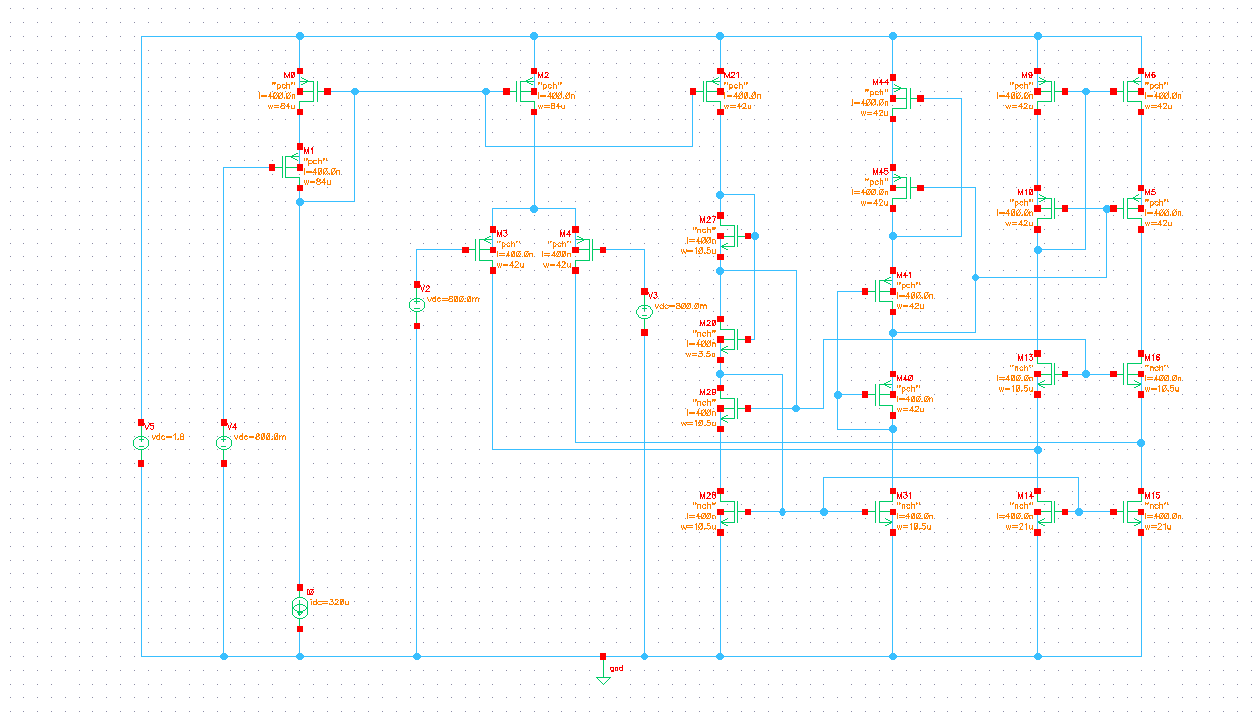
\includegraphics[width=6in]{bullet2_schem.png}
\caption{Schematic Diagram for the Folded Cascode OTA with Associated Biasing Circuitry}
\label{b2_schem}
\end{figure}

\begin{figure}[H]
\centering
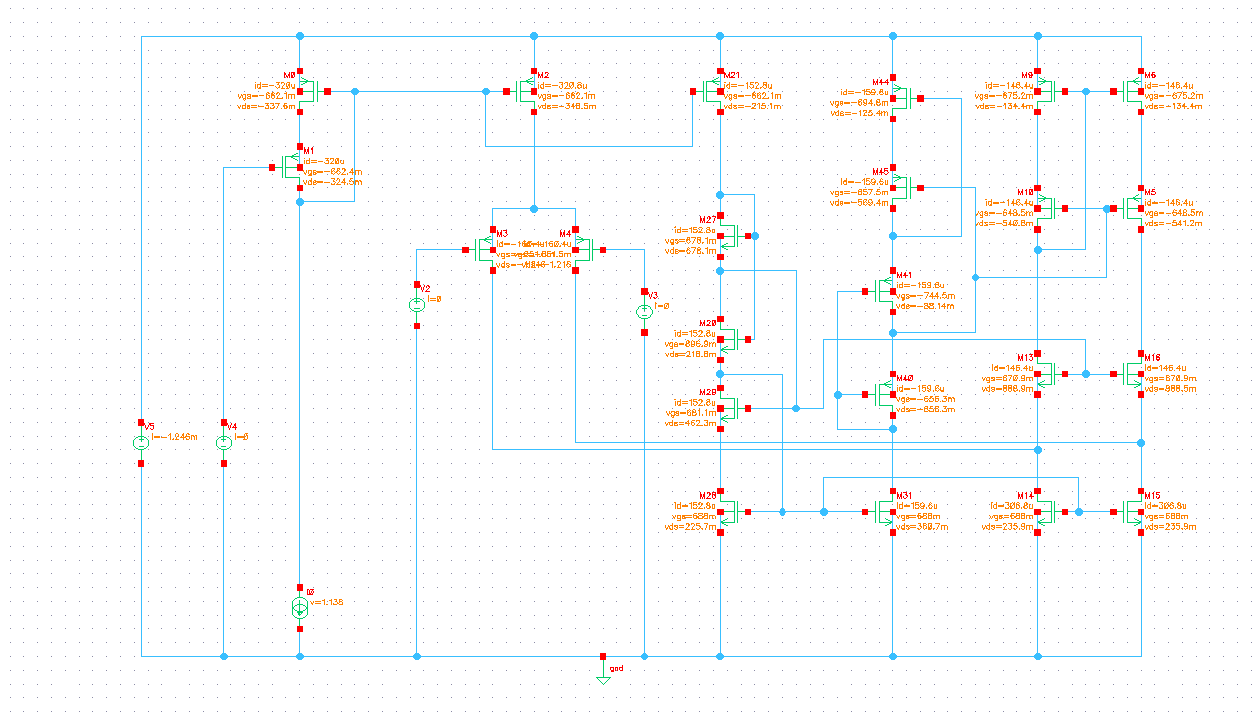
\includegraphics[width=6in]{bullet2_dcop.png}
\caption{Schematic Diagram for the Folded Cascode OTA with Annotated DC Operating Point Values}
\label{b2_dcop}
\end{figure}
\newpage

\section{Bullet Point 3}
I performed a DC sweep of $V_{out-OL}$ against $V_{in-OTA}$ with the OTA in stand alone and the expected transfer function for a differential amplifier is attained (see Figure \ref{b3}).

\begin{figure}[H]
\centering
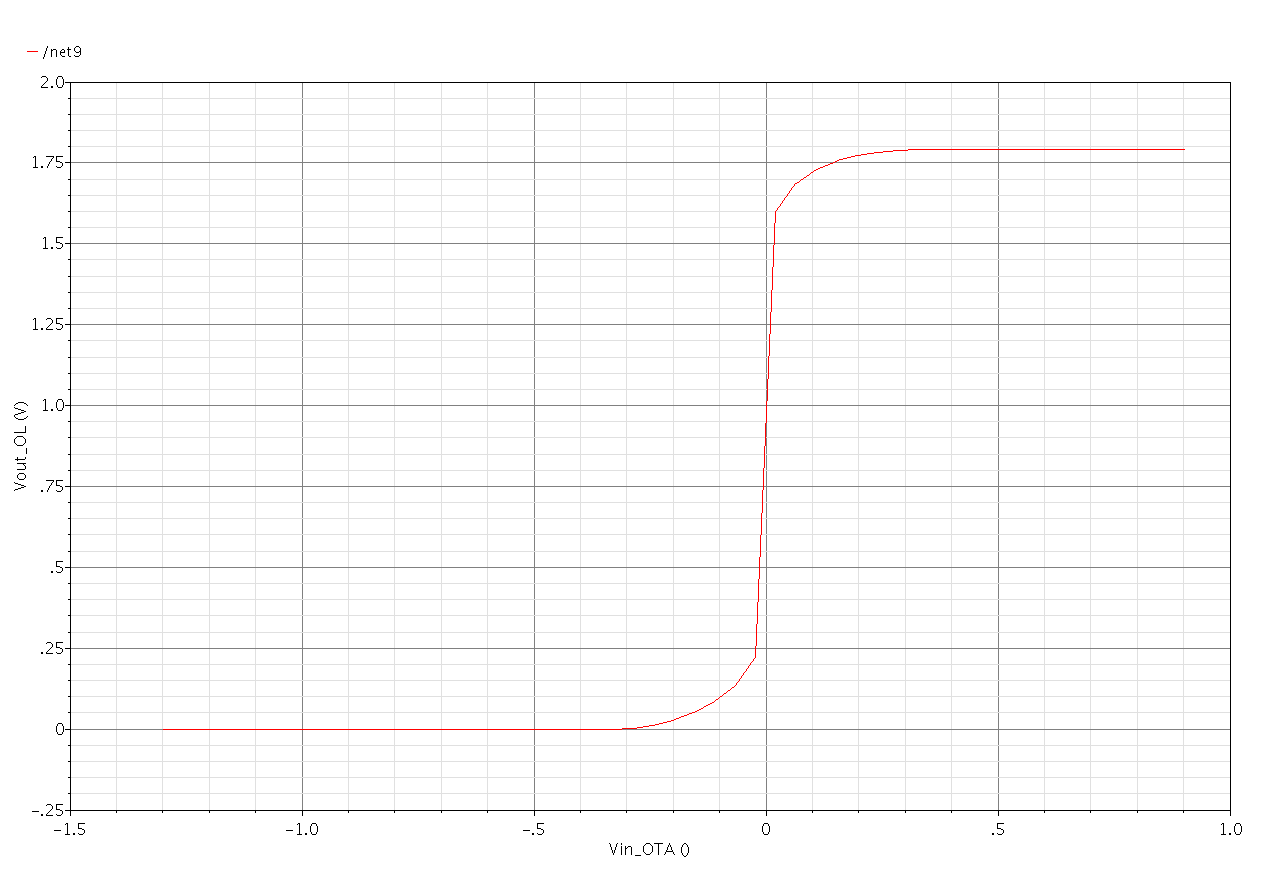
\includegraphics[width=6in]{bullet3.png}
\caption{Voltage Transfer Characteristic for the Folded Cascode OTA in Stand Alone}
\label{b3}
\end{figure}
\newpage

\section{Bullet Point 4}
I applied a small-signal differential input as well as some DC feedback circuitry in order to simulate the open loop gain. Because the open loop gain does not consider small signal feedback, I wanted to build a  circuit that would block all AC feedback. However, I wanted to use this feedback to bias $V_{cm}$. To do this I implemented an RC lowpass filter with a negligible cutoff voltage as can be seen in Figure \ref{b4_schem}. I performed an AC simulation of the open loop gain of the circuit (see Figure \ref{b4_bode}) and was able to attain $A(s) = 521.19\frac{V}{V} = 54.34dB$. Please note that since transistor M44 does not directly affect the biasing, I was able to reduce its size to $~16\mu A$ and optimize my gain.

From the phase plot of my optimized open loop circuit (Figure \ref{b4_bode}), I estimate that there are poles at $~227kHz$ and $471MHz$ and a zero at 945MHz. I estimate the gain-bandwidth product (taken at -3dB from the maximum gain) to be $~72.2MHz$.

\begin{figure}[H]
\centering
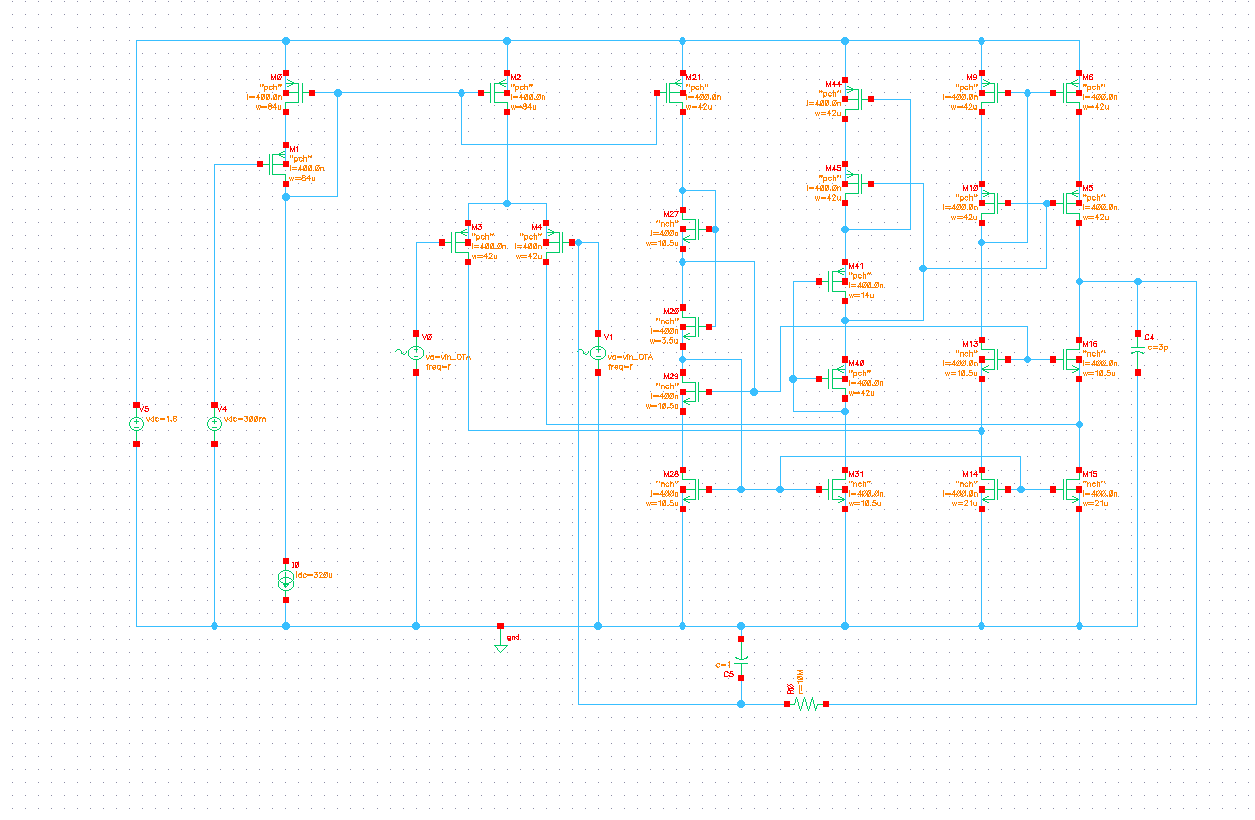
\includegraphics[width=7in]{bullet4_schem.png}
\caption{Schematic Diagram for the Folded Cascode OTA for Open Loop Gain Simulation}
\label{b4_schem}
\end{figure}

\begin{figure}[H]
\centering
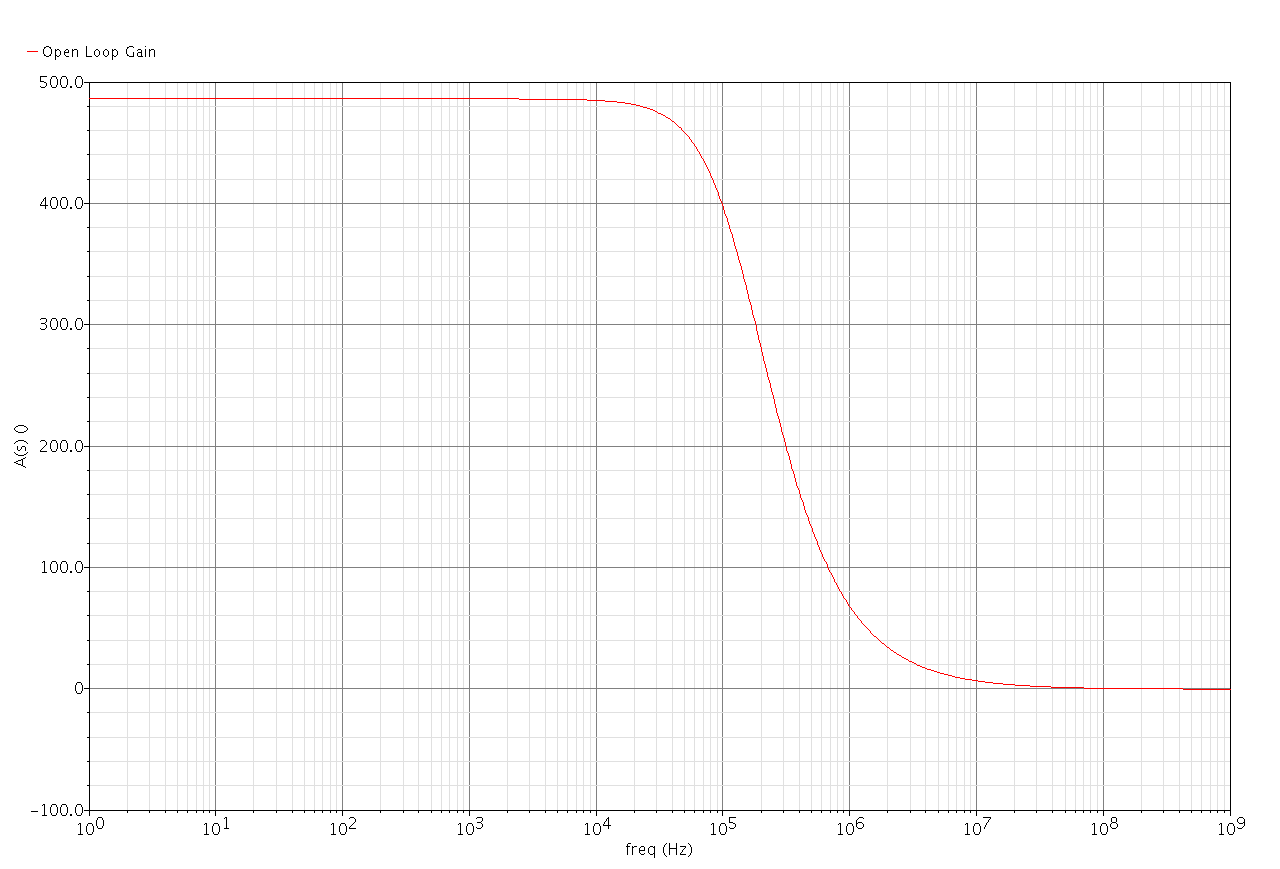
\includegraphics[width=7in]{bullet4_bode.png}
\caption{Bode Plot of the Open Loop Gain of the OTA}
\label{b4_bode}
\end{figure}
\newpage

\section{Bullet Point 5}
INSERT SCAN HERE

\section{Bullet Point 6}
I placed my OTA in AC feedback as shown in Figure \ref{b6_schem} with $V_{cm} = 0.8V$. To find the feedback factor, $\beta$, from this configuration, I plotted the current through the feedback resistor over the voltage at the output (see Figure \ref{b6_beta}).

\begin{equation}
\beta = \frac{I_f}{v_{out}}
\end{equation}

From my simulation, I attained a value of $\beta = 0.577mA/V$. This is comparable to the ideal value of

\begin{equation}
\beta_{ideal} = \frac{1}{R_f} = 0.4mA/V
\end{equation}

\begin{figure}[H]
\centering
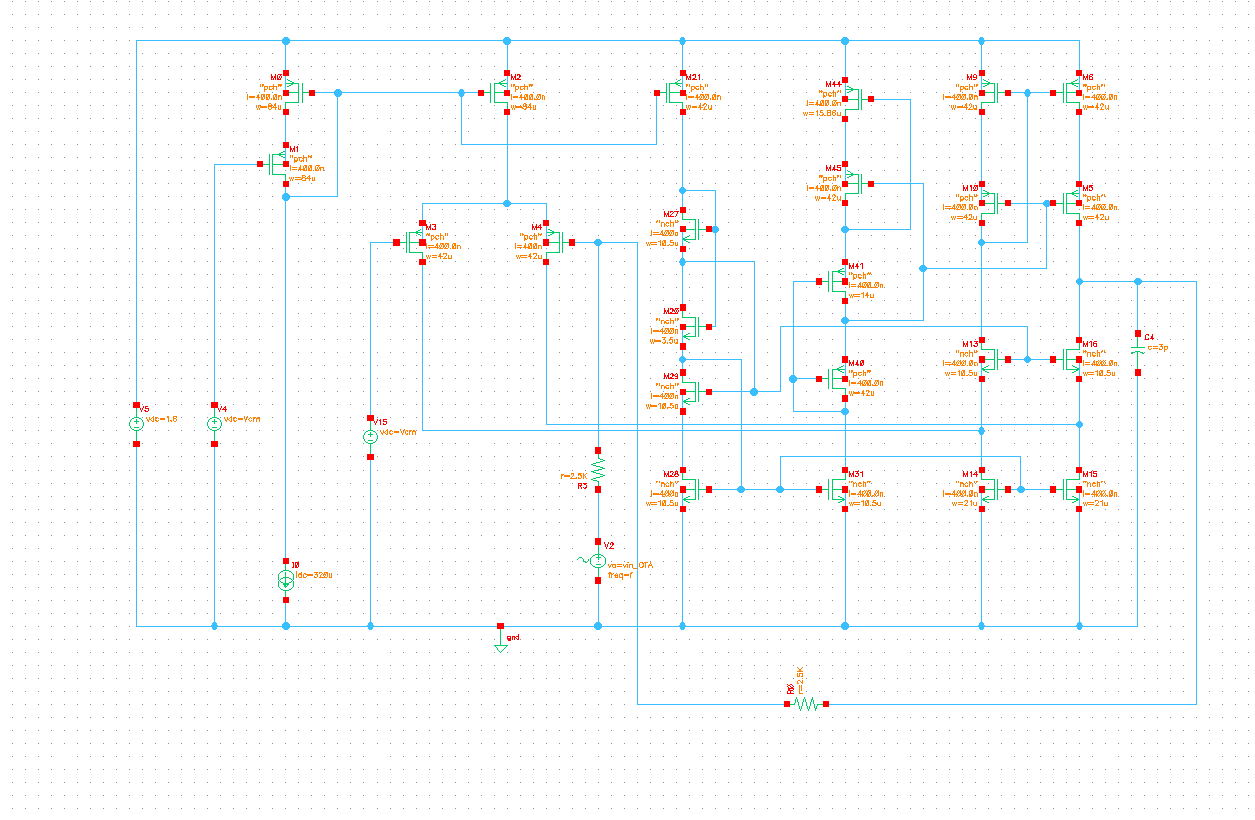
\includegraphics[width=7in]{bullet6_schem.png}
\caption{Schematic Diagram for the Folded Cascode OTA for Closed Loop Gain Simulation}
\label{b6_schem}
\end{figure}

\begin{figure}[H]
\centering
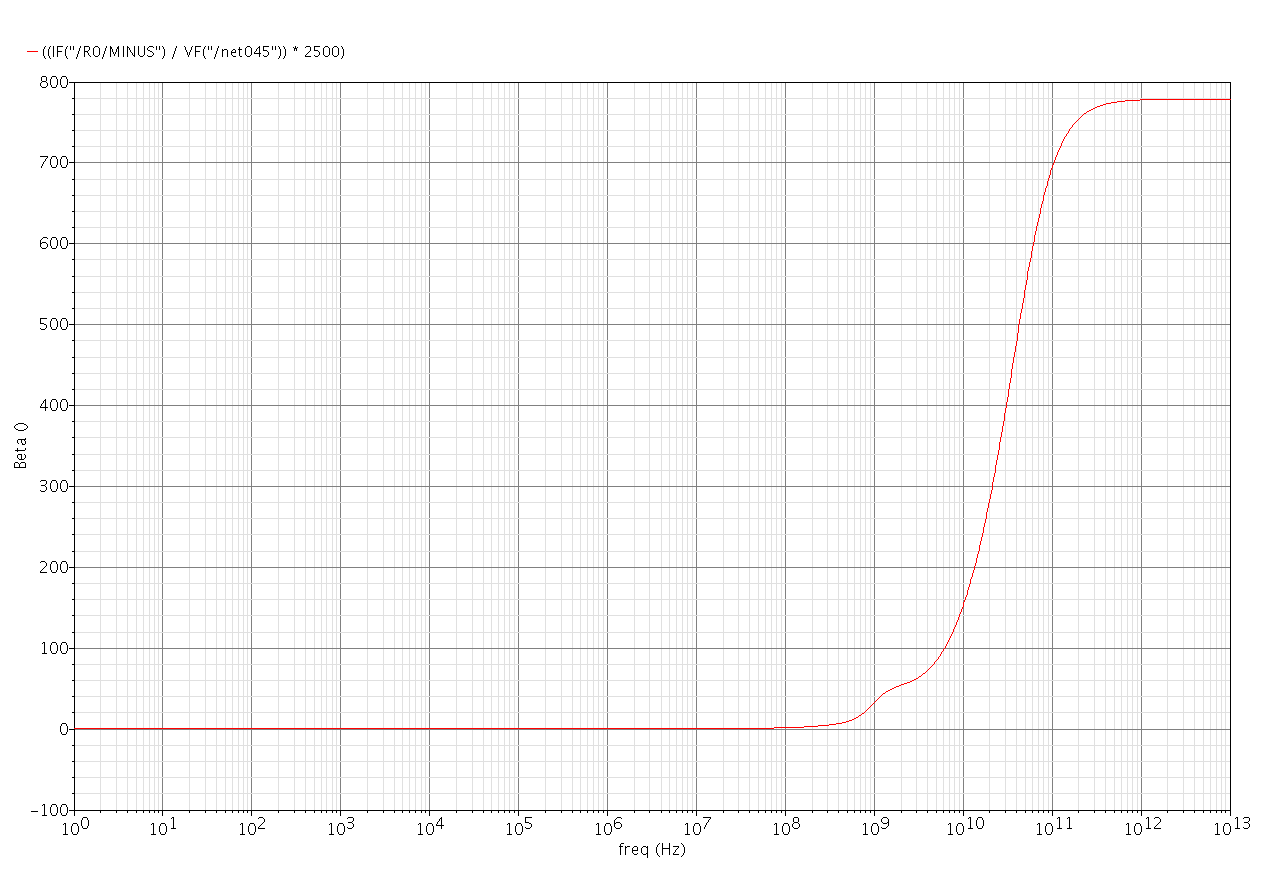
\includegraphics[width=7in]{bullet6_beta.png}
\caption{Frequency Response of the Feedback Network}
\label{b6_beta}
\end{figure}

\section{Bullet Point 7}
\section{Bullet Point 8}
\section{Bullet Point 9}
\section{Bullet Point 10}
With an ideal op-amp (infinite gain and bandwidth), a small-signal step at the input should cause an immediate small-signal step at the output. The reason for this is that with infinite bandwidth, $\tau$ is defined as

\begin{equation}
\tau = \frac{1}{2\pi f_{3dB}} = \infty.
\end{equation}

To determine the output function, we use the equation

\begin{equation}
v_{OUT} = \mu (t) \{1-e^{\frac{-t}{\tau}}\} = \mu (t).
\end{equation}

Therefore, with a small-signal step function at the input, we will observe a small-signal step function at the output.
\newpage

\section{Bullet Point 11}
To determine the ideal output step for the various small-signal step inputs, I first had to simulate the closed loop gain of my circuit. To do this I constructed the circuit shown in Figure \ref{b11_gainschem} and acquired a gain of $A_{closed-loop} = 0.53V/V = -5.51dB$ (see Figure \ref{b11_gain}). I then set out to simulate the step response at various input magnitudes and sample at times $2\tau$ and $100Ts$. My transient step responses can be seen in Figure \ref{b11_step} and my voltage transfer characteristic for $V_{ideal}, V_{out1},$ and $V_{out2}$ can be seen in Figure \ref{b11_transfer}.

The absolute and percent errors are shown in the Chart \ref{b11_errors}.

\begin{figure}[H]
\centering
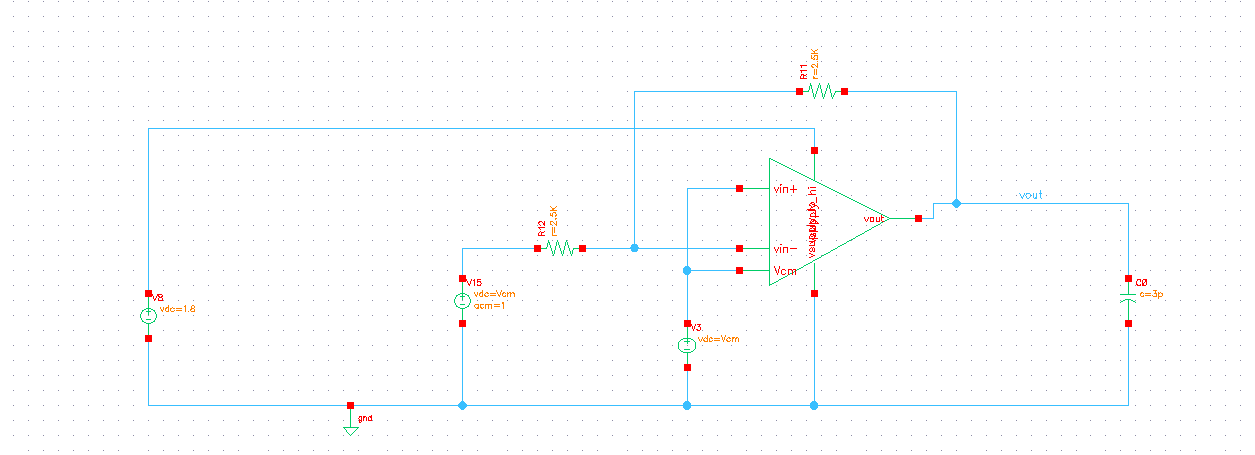
\includegraphics[width=7in]{bullet11_gainschem.png}
\caption{Schematic to Measure Closed Loop Gain}
\label{b11_gainschem}
\end{figure}

\begin{figure}[H]
\centering
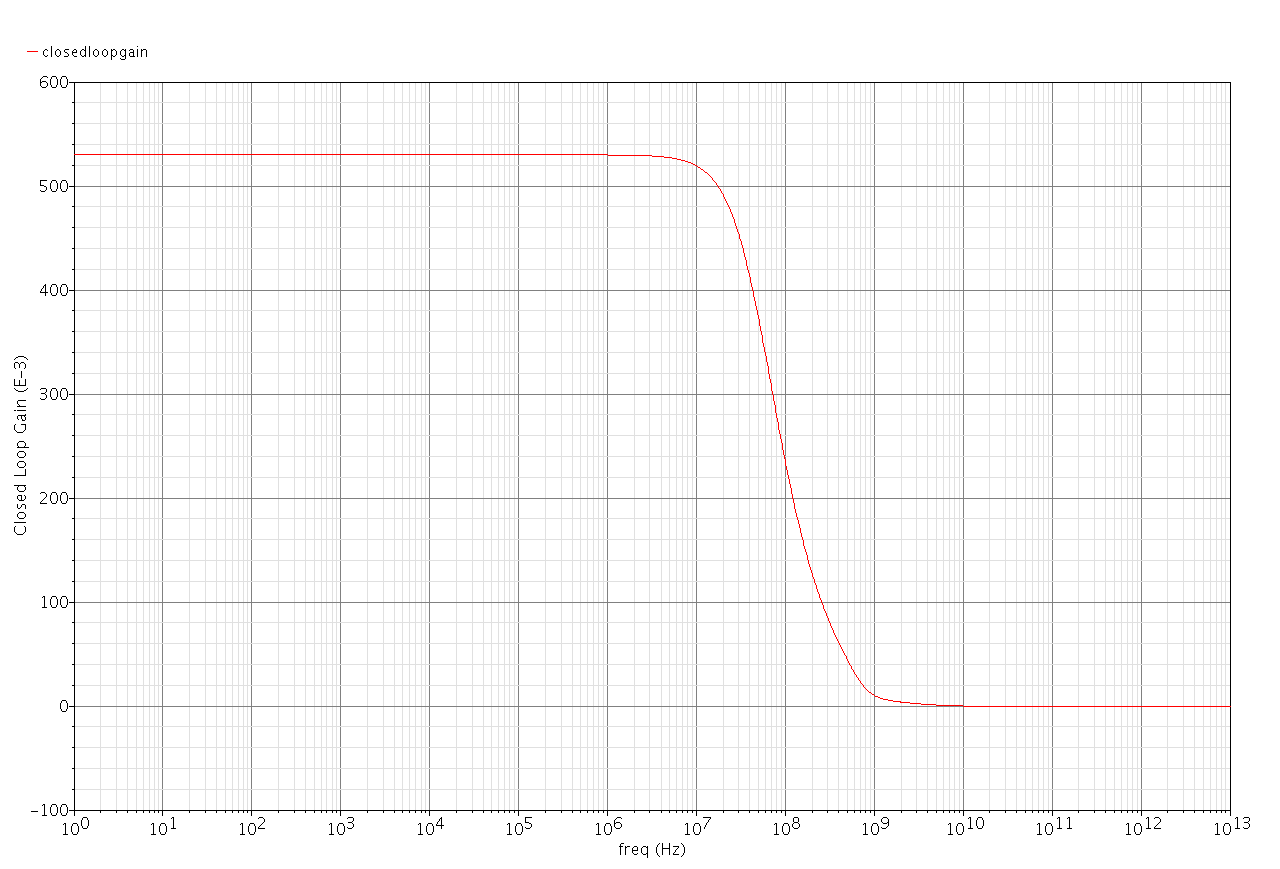
\includegraphics[width=5.5in]{bullet11_gain.png}
\caption{Closed Loop Frequency Response of the OTA in Feedback}
\label{b11_gain}
\end{figure}

\begin{figure}[H]
\centering
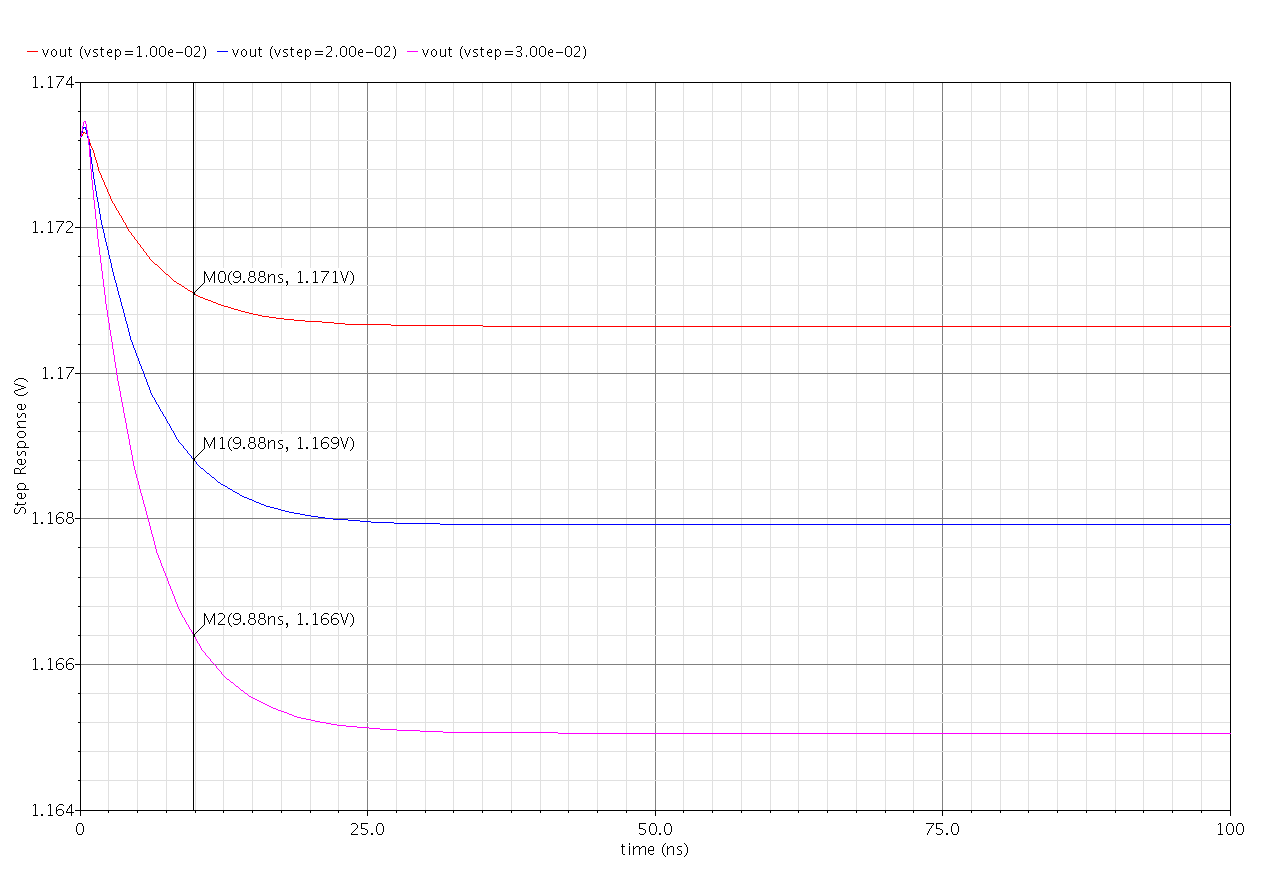
\includegraphics[width=5.5in]{bullet11_step.png}
\caption{Step Responses for Various Small-Signal Input Step Sizes}
\label{b11_step}
\end{figure}

\begin{figure}[H]
\centering
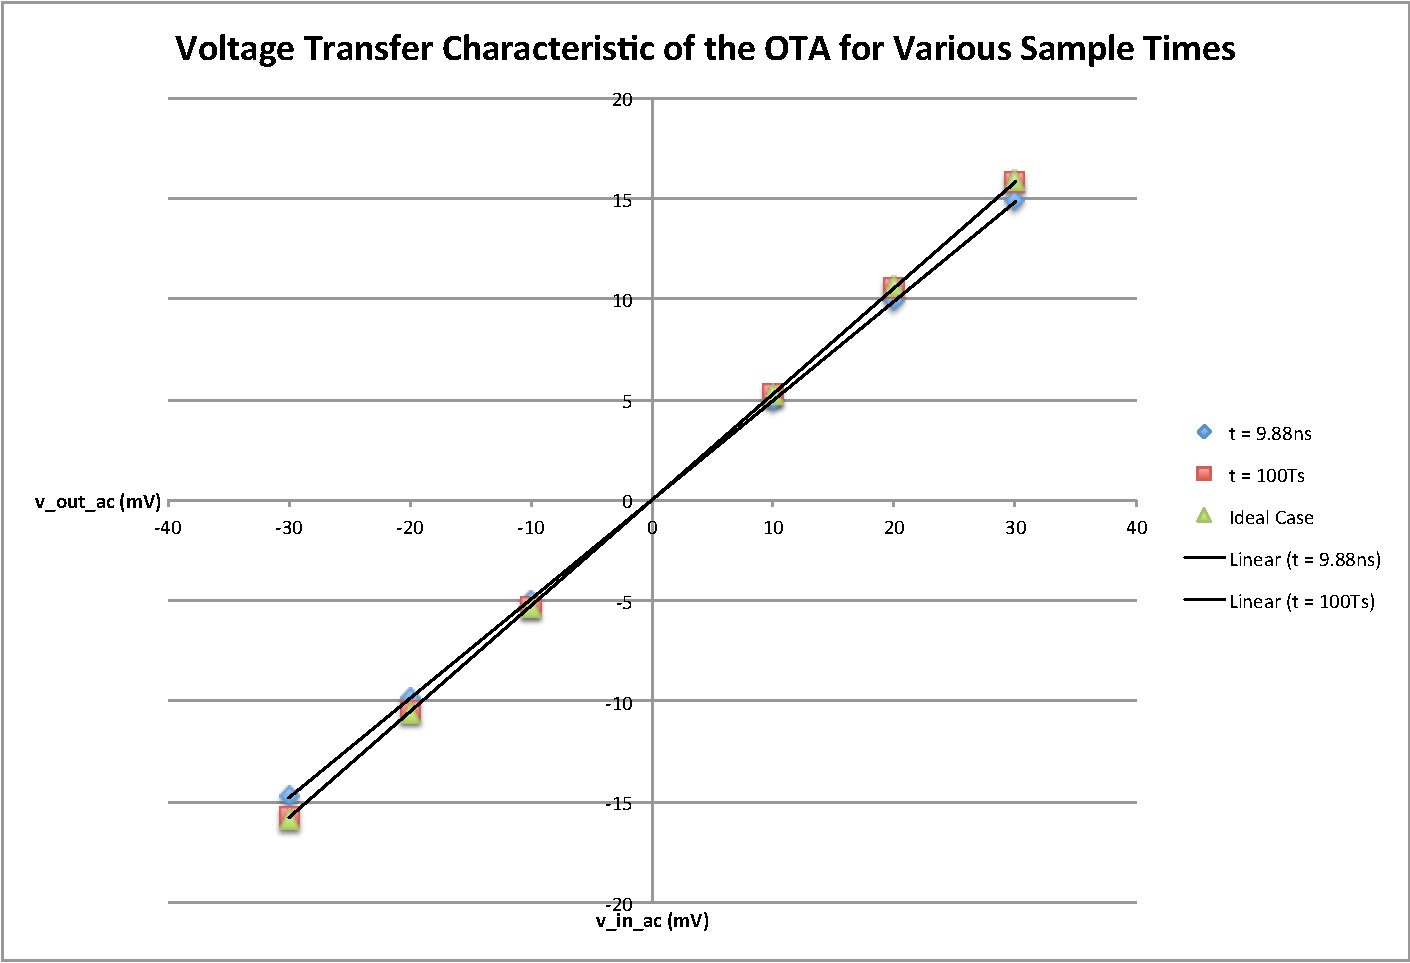
\includegraphics[width=5.5in]{bullet11_transfer.pdf}
\caption{Transfer Function of the OTA Step Response}
\label{b11_transfer}
\end{figure}

\begin{table}[H]
\centering
\newcolumntype{R}{>{\centering\arraybackslash}X}
\begin{tabularx}{500pt}{|R|R|R|R|R|R|}
\hline
$v_{in} [\unit{}{mV}]$&$v_{ideal} [\unit{}{mV}]$&Absolute Error at $t = 2\tau[\unit{}{mV}]$&Percent Error at $t = 2\tau[\unit{}{\%}]$&Absolute Error at $t = 200Ts[\unit{}{mV}]$&Percent Error at $t = 200Ts[\unit{}{\%}]$\\ \hline
10&5.30&0.33&6.17&0.03&0.51\\ \hline
20&10.60&0.71&6.70&0.05&0.47\\ \hline
30&15.90&1.06&6.67&0.07&0.44\\ \hline
-10&5.30&0.31&5.89&0.04&0.79\\ \hline
-20&10.60&0.74&7.00&0.08&0.82\\ \hline
-30&15.90&1.15&7.23&0.14&0.86\\ \hline
\end{tabularx}
\caption{Error Values for Small Signal Step Response}
\label{b11_errors}
\end{table}

\section{Bullet Point 12}
\section{Bullet Point 13}
I extended my step response plot for input steps of $\pm 100mV$, $\pm 200mV$, and $\pm 500mV$ to show the effects of slewing. As can be seen in Figure \ref{b13_step}, slewing is most obvious in the 500mV response.

\begin{figure}[H]
\centering
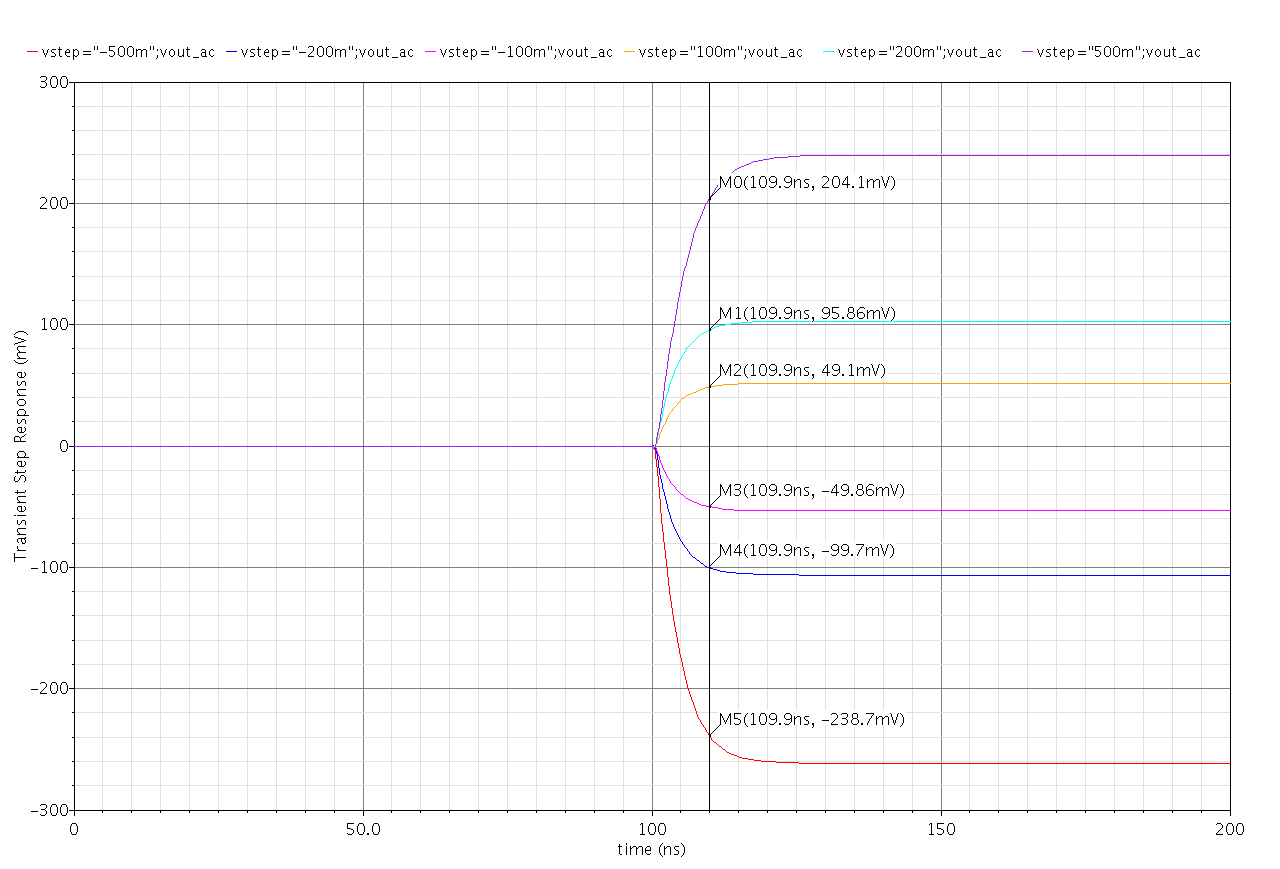
\includegraphics[width=5.5in]{bullet13_step.png}
\caption{Step Responses for Various Large-Signal Input Step Sizes}
\label{b13_step}
\end{figure}


\end{document}
